\chapter{AI Algorithms and Architectures}
Before describing what techniques can be used to implement an AI system which plays backgammon, it is important to describe the game itself.

Backgammon is a two player, zero sum game with chance and perfect information.
\begin{definition}[Zero sum]
One player's advantage is equivalent to another player's loss. The sum of the player's scores is always zero.

Example: Chess

Non-example: Cooperative games
\end{definition}

\begin{definition}[Perfect information]
    Both players have complete knowledge of the game state at all times. There is no hidden information.

    Example: Checkers

    Non-example: Poker
\end{definition}

\begin{definition}[Chance]
    There is an element of randomness in the game.

    Example: Go

    Non-example: Snakes and Ladders
    
\end{definition}

For such games, the best systems (such as AlphaGo) used a trained policy network (using neural networks), combined with Monte Carlo Tree Search (MCTS) in real-time gameplay \cite{aiparadigms} \cite{alphago}.
MCTS is limited to games with perfect information, and also requires that the action space (the set of all moves a player can make) is discrete, which are both true for backgammon.

Game trees are often used to represent the states and moves in a game. Each node represents a game state, and each edge represents a move which the player can make. The root node corresponds to the current state of the game. Leaf nodes represent terminal positions (wins, losses, and draws). An example game tree for tic-tac-toe is shown in figure \ref{fig:gametree}. This representation allows tree traversal algorithms to be used to analyse different properties of a state and its corresponding moves, such as the expected value.

\begin{definition}[Branching Factor]
    The average number of possible states which can be reached from the current state.    
\end{definition}

\begin{figure}[H]
    \centering
    \includegraphics[width=0.7\linewidth]{images/gametree.png}
    \caption{Partial Game Tree for Tic-Tac-Toe \cite{tictactoe}}
    \label{fig:gametree}
\end{figure}



This project includes different types of AI systems that can be used to play backgammon, such as rule-based systems, neural networks, and MCTS.

\section{Heuristics}
Heuristic approaches involve estimating the value of a given board state using rules which have been shown to work through trial and improvement. These rules typically combine several features based on expert knowledge, such as pip count difference (a measure of race progress TODO add to definitions), number of blots, strength of primes, control of anchors, and how widely checkers are spread \cite{heuristic}. The agent then selects the move leading to the state with the best heuristic evaluation. While intuitive, designing effective heuristics can be complex, and heuristic rules may struggle with the nuances and dynamic nature of the game.


\section{Stochastic Gradient Descent (SGD)}
While heuristic evaluation functions provide a computationally cheap way to estimate the strength of a board position, manually tuning the weights associated with different features can be challenging, subjective, and may lead to suboptimal performance. SGD offers an automated method for learning these weights based on game experience.

The heuristic function $H(s, \textbf{w})$ calculates the value of state $s$ as a linear combination of features $f_i(s)$ with corresponding weights $w_i$. The goal of SGD is to find the optimal weights $\textbf{w}$ such that $H(s, \textbf{w})$ gives the most accurate estimate for the value of a given state.

A loss function is used to measure how good a particular action is, by comparing the estimated outcome to the actual outcome of the game $T$. Commonly, a value of +1 is used to represent a win, and -1 for a loss. The difference between the heuristic prediction and the target outcome can then be defined using the mean squared error:
$$
L(\textbf{w}) = E[(T - H(s, \textbf{w})^2]
$$
where $E[...]$ denotes the expectation over all possible states during the game.


The goal of SGD can be redefined as minimising the loss function $L(\textbf{w})$.

Gradient descent algorithms work by iteratively updating the values of $\textbf{w}$ by moving the values of $\textbf{w}$ in the opposite direction of the gradient. This results in the following update rule:
$$
\textbf{w} \leftarrow \textbf{w} - \eta \nabla L(\textbf{w})
$$
where $\nabla L(w)$ is the gradient of $L(w)$ and $\eta$ is the learning rate, a value that determines the size of the steps the update rule makes. As shown in figure \ref{fig:gradientdesc}, by moving in the direction of the negative gradient, the points converge to a local minimum of the function, and may not find the global minimum.

\begin{figure}[H]
    \centering
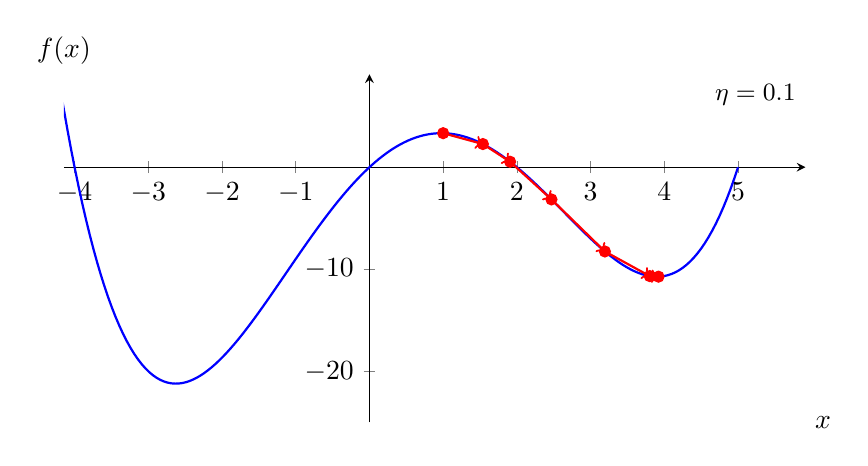
\begin{tikzpicture}
  \begin{axis}[
      domain=-5:5, samples=200,
      xlabel=$x$, ylabel=$f(x)$,
      axis lines=middle,
      ymin=-25, ymax=6,
      width=11cm, height=6cm,
      enlargelimits=upper,
      every axis y label/.style={at={(0,1)},anchor=south},
      every axis x label/.style={at={(1,0)},anchor=west}
    ]

    %% --- the objective f(x)=1/6*(x^4 - 3x^3 - 18x^2 + 40x) ---
    \addplot[blue, thick] {1/6*(x^4 - 3*x^3 - 18*x^2 + 40*x)};

    %% ---- descent points (x_n, f(x_n)) ----
    \addplot[only marks, mark=*, mark size=2pt, red]
      coordinates {
        (1.000,  3.333)   % x0
        (1.539,  2.268)   % x1
        (1.908,  0.536)   % x2
        (2.469, -3.158)   % x3
        (3.194, -8.260)   % x4
        (3.802, -10.673)  % x5
        (3.921, -10.729)  % x6 ≈ local min
      };

    %% --- arrows between successive points (gradient steps) ---
    \draw[->, red, thick] (axis cs:1.000, 3.333)   -- (axis cs:1.539, 2.268);
    \draw[->, red, thick] (axis cs:1.539, 2.268)   -- (axis cs:1.908, 0.536);
    \draw[->, red, thick] (axis cs:1.908, 0.536)   -- (axis cs:2.469, -3.158);
    \draw[->, red, thick] (axis cs:2.469, -3.158)  -- (axis cs:3.194, -8.260);
    \draw[->, red, thick] (axis cs:3.194, -8.260)  -- (axis cs:3.802, -10.673);
    \draw[->, red, thick] (axis cs:3.802, -10.673) -- (axis cs:3.921, -10.729);

    %% --- annotate the learning rate ---
    \node[anchor=north east,font=\small]
      at (axis description cs:1,1) {$\eta=0.1$};

  \end{axis}
\end{tikzpicture}






    \caption{Gradient Descent Algorithm used on $f(x)=\frac 16(x^4 - 3x^3 - 18x^2 + 40x)$ with a learning rate of $\eta = 0.1$}
    \label{fig:gradientdesc}
\end{figure}


The problem with this is calculating the gradient of the loss function requires summing over the entire distribution of states, which is computationally intractable. SGD overcomes this limitation by estimating the true gradient using only a few training examples at each step. This is both much more computationally efficient, and also has the added benefit of helping to escape local maxima \cite{sgdescape}. 

Over many iterations, these adjustments will move the weights $\textbf{w}$ towards the value that minimises the prediction error, i.e. the value which results in the heuristic function being as accurate as possible at predicting the value of a given state \cite{sgd}.


\section{Monte Carlo Tree Search}
\label{sec:mcts}
Monte Carlo methods are a type of algorithm that estimates an unknown value based on random sampling. They are often used to solve problems that are deterministic in principle but difficult or impossible to solve with exact analytical methods \cite{RussellNorvig}. For example, calculating a complete game tree of backgammon and picking the best child node could theoretically be calculated, but is computationally intractable. By generating many random samples and observing the outcomes, Monte Carlo methods utilise the Law of Large Numbers to approximate solutions.

\begin{definition}[Law of Large Numbers]
    The Law of Large Numbers states that the sample mean of $n$ independent and identically distributed random variables with mean $\mu$ approaches $\mu$ as $n$ tends to infinity.
\end{definition}


Monte Carlo Tree Search (MCTS) is a specific Monte Carlo method which is used to search game trees to find optimal moves. Because of its stochastic nature, it is especially well suited to chance games which have a high branching factor, such as backgammon ~\cite{Browne2012} \cite{mctsbranching}. TODO I think i have written this somewhere previously


Intuition: A game tree is created with the current state as the root node. A child node is chosen and random moves are made by both players until the end of the game or a maximum depth cut off is reached. The results of these games are propagated back throughout the tree and the expected value of each node is updated. By doing this a large number of times, the expected value of each node can be estimated, and the move resulting in the highest expectation can be picked.

The algorithm iteratively runs 4 steps until termination. 
\begin{enumerate}
    \item \textbf{Selection}: Starting at the root node, a child node is chosen according to a tree policy. This policy tries to balance exploring unvisited nodes (which may have high potential), with exploiting nodes which have been shown to be promising.
    \item \textbf{Expansion}: If the selected child node does not represent a terminal game state, it is then added to the stored game tree. 
    \item \textbf{Simulation}: From this newly added node, a simulation is run by randomly choosing moves for both players. This is continued until the end of the game is reached, or until another condition is met, such as reaching a move limit, or reaching a state where calculating the winner can be done easily.
    \item \textbf{Backpropagation}: The outcome of the game is backpropagated throughout the tree, from the expanded node to the root node. The statistics of each node along the path is updated, for example, the expected value of the node, and how many times the node has been visited. 
\end{enumerate}

This cycle is repeated until some condition is met. This could be until a certain amount of time has elapsed, or a predetermined number of simulations has been reached. Finally, a move is chosen from the children of the root node. This is could be the node with the highest estimated value, or the node with the highest visit count.

TODO move to implementation: Due to backgammon's large branching factor, nodes have a large variance in their expected values. It is therefore important to maximise the number of rollouts to reduce the error of estimations as much as possible. something like "the main goal when implementing MCTS is to make it as fast as possible".
TODO also move to implementation: TODO it is important when implementing this that the number if simulations is high enough so that ... If this is not the case, the likelihood of the grandchild node being computed will be low (or will have low N TODO). Due to the time taken searching the game tree for the grandchild, the agent will have less time to do further rollouts, which will result in worse performance. 

There are many enhancements that can increase the performance of MCTS, many of which are described in ``A Survey of Monte Carlo Tree Search Methods" \cite{Browne2012}. Some enhancements which are more applicable to backgammon are listed below.

\begin{definition}[Exploration-exploitation trade off]
    The problem of balancing choosing the best path based on current knowledge (exploitation), and choosing new paths which have the possibility of better outcomes (exploration).
    
\end{definition}

\begin{itemize}
    \item One obvious improvement is to reuse subtrees that have been previously computed. When an updated board has been passed to the algorithm, the previous tree can be searched to find the node corresponding to the new state. By setting this node to be the root, less time is spent rebuilding layers of the tree from scratch, visit counts and value estimates are preserved, and statistics are more accurate.  
    
    \item UCB1-Tuned \cite{monteCarloImprovements} \cite{banditproblem}: One of the main problems in implementing Monte Carlo Tree Search is choosing the tree policy for selection. The tree policy needs to balance the exploration-exploitation trade off. UCB1-tuned offers a tigher bound compared with the more commonly used UCB1 algorithm \cite{ucb1tuned}. When choosing which child node to explore, UCB1-tuned chooses the child which maximises the value.
    \begin{equation}
        \mathrm{UCB} 1 \text{-Tuned}=\bar{X}_j+2C\sqrt{\frac{\ln n}{n_j} \min \left\{\frac{1}{4}, V_j\left(n_j\right)\right\}}
        \label{eq:ucb1}
    \end{equation}
    
    
    where 
    $$
    V_j(s)=\left(1 / 2 \sum_{\tau=1}^s X_{j, \tau}^2\right)-\bar{X}_{j, s}^2+\sqrt{\frac{2 \ln t}{s}}
    $$ in the case that child node $j$ has been chosen $s$ times in the first $t$ simulations, $\bar{X_j}$ is the average reward of child node $j$, $n$ is the total number of simulations, $n_j$ is the number of times node $j$ has been chosen already, and $C$ is a constant exploration parameter (where a higher value of C results in more exploration). 
    
    The first term $\bar{X_j}$ represents ``exploitation", where a higher expected value will result in the node being picked more often, while the other term represents the ``exploration" term, where values which have been picked a lower proportion of the time have a higher value.
    This policy increases the rate of convergence by using the observed variance to scale the exploration term.

    \item Rapid Action Value Estimation (RAVE): RAVE is a popular method for improving the information stored in each nodes statistics, particularly in Go programs, which leads to faster convergence during the early stages of search \cite{GellySilver2007}. For each move, statistics across all simulations where that move appears is updated, with the assumption that a move that performs well in one state is likely to perform well in other similar states. The RAVE value is then combined with UCB values to estimate a nodes value.


    \item Combining MCTS with other models \cite{44806} \cite{Browne2012}: 
    One of the biggest improvements that have been made in MCTS agents is the integration of policy networks to select moves and value networks to evaluate board positions. 
    By using a policy network, nodes with lower value can be quickly identified and do not need to be expanded.
    By using a value network, games to not need to be expanded to the end.
    Instead the simulation is run to a predetermined depth, at which point the value network is used to evaluate the board position.
    Since the value network will be provided boards which are closer to the end of the game, it will be able to provide a more accurate estimate of the value of the board position compared to a pure network agent.
    By terminating simulations early, more iterations of MCTS can be performed, increasing performance. The most notable example of this is AlphaGo, which used a combination of MCTS, policy networks, and value networks to achieve superhuman performance in Go, achieving a 99.8\% winrate against other Go programs \cite{44806}.
 
\end{itemize} 

\subsection{Predicting Win Probabilities}
Ross, Benjamin, and Munson present a closed form approximation for the probability that a player wins a backgammon race \cite{estimating}.
By using the Raw Pip Count (RPC) of each player, a Single Checker Model (SCM) is created, which approximates each player's position as a single checker which needs to travel a distance equal to the RPC.
An existing approximation based on the central limit theorem is then used to estimate the SCM probabilities. 

\begin{definition}[Central limit theorem]
The sample mean $\bar X_n $of $n$ indepdendent and identically distributed values approaches the population mean $\mu$ and has a distribution of $\bar X_N \sim N(\mu, \frac{\sigma^2}{n})$ where $\sigma$ is the population variance.    
\end{definition}


After comparing this approximation of to simulations of real backgammon races, the formula was adjusted to account for bearing off rules and pip wastage, which the original SCM approximation did not take into account. This leads to the following value:
\begin{equation}
\label{eq:d2s}
    \frac{\Delta^2 + \Delta / 7}{S - 25}
\end{equation}


where $\Delta = Y - X + 4$ is the adjusted difference in RPC between the two players, and $S = X + Y$ is the sum of the two players RPCs, where $X$ is the lower pip count, and $Y$ is the higher pip count of the two players. 
This value is then compared with a precomputed lookup table to determine an approximate probability of winning the race (and therefore the game). TODO add table to appendix.
This model was originally designed to be used by players to estimate the probability of winning during the game using only mental arithmetic, and therefore has a number of limitations. The model does not take into account hitting or any other interactions between checkers, such as when a player is blocked, and some simplifications to the formula were made so players could easily calculate values mentally.


\section{Neural Networks} 

A neural network is a computational model which maps inputs to outputs using a series of transformations.
In particular, multilayer perceptron (MLP) models consists of an input layer, one or more hidden layers, and an output layer, where each layer is made up of interconnected nodes (neurons) that calculate a weighted sum of its inputs, and applies a non-linear activation function to produce an output. 
The universal approximation theorem states that a large enough MLP can approximate any continuous function to arbitrarily high accuracy \cite{Hornik1989}.
In the context of backgammon, the input layer would represent a board state, and the output layer would represent the probability of winning from that state.
In a deep neural network, only the board state is passed to the first layer, and the higher level features would be learned by the network as it is trained, however this requires a large amount of training and computation. 
A simpler approach is to use a network with less neurons and less layers, thus needing less training data and computation, and passing in the features of the board state as inputs.

Training a neural network involves adjusting its weights so that its outputs match the desired targets on a set of training examples. This is done by minimising the difference between the network's prediction and the desired output value.

At each iteration, the gradient of the loss function with respect to the weights is computed, and the parameters are updated in the direction that decreases the loss function.

 The backpropagation algorithm is used to compute the gradients by applying chain rule as follows:

\begin{enumerate}
  \item \textbf{Forward pass:} For each training example, the input is passed through each layer of the network.
  \item \textbf{Compute loss:} The loss function is evaluated using the network's final output and the true target.
  \item \textbf{Backward pass:} Starting from the output layer, the error term for each layer is computed. The gradients of the loss with respect to the weights in each layer is then calculated, which involves multiplying the derivatives of the error from previous layers. 
  \item \textbf{Parameter update:} Using gradient descent, the weights of each neuron are adjusted.
\end{enumerate}


\section{Reinforcement Learning}
Reinforcement learning is a type of machine learning where an agent learns by interacting with an environment to maximise reward, as opposed to learning from labelled inputs and outputs (supervised learning) or learning from unlabelled data (unsupervised learning). By taking actions in an environment and observing the outcome, the agent is able to choose actions which maximise the reward.  
One technique for training an agent using reinforcement learning is to implement self-play, where the agent plays against itself repeatedly and learns from the outcomes. 
As backgammon naturally has chance, the agent is forced to explore a wide variety of boards, which helps to avoid the problem of converging to a local minimum instead of the global minimum. 
This is unlike with stochastic gradient descent for two reasons: first, the neural network learns from every board state, while SGD learns only from the outcome; second, the neural network aims to learn the value of a board state, while SGD aims to learn a strategy for playing the game i.e. the neural network needs to see different positions to learn (which is natural to backgammon), while SGD needs to play against different styles to learn. 

From this, an initial model could be created which learns in the following way:
\begin{enumerate}
    \item The agent plays a game against itself, and the final outcome is recorded.
    \item The neural network is trained on every board state it has seen in the game, using the final outcome as the target value for each board state.
    \item The agent continues to play against itself and learn from the outcomes until some point is reached, such as a certain number of games have been played or a certain accuracy is reached.
\end{enumerate}

The problem with this approach, is that by assigning each board state the same value, the implicit assumption is that all moves are equally important, which is not the case and causes the network to overestimate the value of early game states.
For example, if the agent makes losing moves for the entire game, but the opponent makes a critical error in the final few moves, the agent will be rewarded for all the states, reinforcing bad moves.

To overcome this, temporal difference learning (TD learning) was developed, which was described by Sutton and Barto as ``one idea central and novel to reinforcement learning" \cite{Sutton2018}.
The way TD learning overcomes this problem is by updating values at each time step based on the expected future rewards (multiplied by some factor $\gamma$), rather than just the final outcome. This comes with two main benefits:
\begin{itemize}
    \item By updating at every step rather than once at the end of the game, the agent is able to identify good and bad moves, and assign rewards accordingly.
    \item The agent is able to learn continuously after every action, rather than waiting until the end of a game to learn.
\end{itemize}
The reason expected future rewards are decayed by $\gamma$ is because rewards become less valuable the longer a player has to wait for them. 
The longer the wait times, the more variance there is in the outcome, and the more likely it is that there will be errors. 
By having a decay factor, the agent is encouraged to take shorter, more certain paths to the goal.

This raises another problem, which is that initially during learning, only terminal states have a non-zero reward, so all intermediate states are not updated until the end of a game, resulting in extremely slow learning.
The idea of TD-$\lambda$ is to solve this problem by updating the value of every past state in a sequence (called an eligibility trace) that led to the reward.
A value is chosen for $\lambda$ between 0 and 1, which determines the decay of the reward, with higher values giving more weight to earlier states.

When state $s$ receives a reward $x$ at time step $t$, the value of previous states $s_{t-1}, s_{t-2}, ...$ are given a reward of $x (\lambda \times \gamma)^{t - i}$, where $i$ is how many steps back the state was seen.

Famously, TD-$\lambda$ was used in TD-Gammon \cite{Tesauro1995}, which was the first backgammon program to achieve expert level play.
It worked by using an MLP to predict the outcome of a game from the given board position. 
When making a move, the program generated all legal moves from the current position, and used the network to evaluate each possible position.
The move with the highest predicted value was then chosen.

During training, the network started from a random initial state and played against itself over and over. 
As training progressed, the network was able to learn basic strategies such as hitting blots, and creating anchors.
TD-Gammon 1.0 contained 198 input nodes and 40 hidden units, and was trained for 200,000 games, resulting in an agent that was able to win regional tournaments.
TD-Gammon 2.1 was close to the world's best players, and was able to discover new strategies which changed how humans play certain board positions.
Pollack and Blair \cite{Pollack1997} suggested that TD-Gammon's success was due to learning through self play, by showing a simpler model which learned effectively through the same method. 



“TD-Gammon has definitely come into its own. There is no question in my mind that its positional judgment is far better than mine.
Only on small technical areas can I claim a definite advantage over it ... Its strength is in the vague positional battles where judgment, not calculation,
is the key. There, it has a definite edge over humans ... In particular, its judgment on bold vs. safe play decisions, which is what backgammon really is all about, is nothing short of phenomenal ...
Instead of a dumb machine which can calculate things much faster than humans such as the chess playing computers, you have built a smart machine which learns from experience pretty much the
same way that humans do”, Kit Woolsey, a top 10 world backgammon player, quoted in ``Temporal Difference Learning and TD-Gammon"\cite{Tesauro1995}.

\section{Ensemble Models}
It is well established in psychology, economics, and other fields that although an individual may be inaccurate in their predictions, the average of many individuals is often more accurate than any one individual, a term referred to as the "wisdom of the crowd" \cite{wisdomjames} \cite{wisdom2}.
This principle can be applied to machine learning, by creating an ensemble of models, where training data is split between multiple models, and the predictions of each model are averaged to create a final prediction \cite{Brown_EnsembleLearning_2011}. 
